\chapter{Introducción}

Hoy en día es muy habitual hacer uso de los sistemas de contenedores, el más conocido es \href{https://docs.docker.com/}{Docker}, en el mundo del desarrollo de \textit{software}. Este sistema trae consigo una serie de ventajas que veremos más adelante, que nos permite asegurar, entre otras cosas, que las versiones utilizadas en el entorno de producción son las mismas que durante las etapas de desarrollo.

En este documento se va a explicar cómo realizar la instalación y configuración de un sistema basado en contenedores Docker para poder arrancar servicios, y ciertas configuraciones que son necesarias conocer.

\chapter{Sistemas de contenedores}

Los sistemas de contenedores son un método de virtualización (conocido como “virtualización a nivel de sistema operativo”), en el que se permite ejecutar sobre una capa virtualizadora del núcleo del sistema operativo distintas instancias de “espacio de usuario”.

Este “espacio de usuario” (donde se ejecutarán aplicaciones, servicios...) se les denomina \textbf{contenedores}, y aunque pueden ser como un servidor real, están bajo un mecanismo de aislamiento proporcionado por el \textit{kernel} del sistema operativo, y sobre el que se pueden aplicar límites de espacio, recursos de memoria, de acceso a disco...

\infobox{\textbf{Un contenedor es un espacio de ejecución de servicios al que se les puede aplicar límites de recursos (como la memoria, el acceso a disco...)}}

Desde el punto de vista del usuario, que un servicio se ejecute en una máquina virtual o en un contenedor es indistinguible. En cambio, desde el punto de vista de un administrador de sistemas o de un desarrollador, el uso de contenedores trae consigo una serie de ventajas que veremos en apartados posteriores.


\section{Un poco de historia}
Aunque está muy en boga el despliegue de aplicaciones haciendo uso de contenedores, no es un concepto nuevo, ya que lleva existiendo desde la década de los 80 en sistemas UNIX con el concepto de \href{https://es.wikipedia.org/wiki/Chroot}{chroot}.

\textbf{Chroot}, también conocido como “jaulas chroot”, permitían ejecutar comandos dentro de un directorio sin que, en principio, se pudiese salir de dicha ruta. Tenía muy pocas restricciones de seguridad, pero era un primer paso al sistema de contenedores.

\href{https://es.wikipedia.org/wiki/LXC}{LXC} nace en 2008 utilizando distintas funcionalidades del kernel Linux para proveer un entorno virtual donde poder ejecutar distintos procesos y tener su propio espacio de red. Con LXC nacen distintas herramientas para controlar estos contenedores, así como para crear plantillas y una \textbf{API que permite interaccionar con LXC} desde distintos lenguajes de programación.

Ha habido otras tecnologías en Linux, como \href{https://es.wikipedia.org/wiki/OpenVZ}{OpenVz}, pero luego nos centraremos en Docker, ya que es lo más conocido actualmente.


\section{Qué es un contenedor y cómo se crea}

Para entender qué es un contenedor dentro de la infraestructura Docker y cómo se crea, tenemos que diferenciar distintos conceptos:
\begin{itemize}
    \item \textbf{Imagen Docker}
    \item \textbf{Contenedor Docker}
\end{itemize}

A continuación se van a detallar en profundidad.

\subsection{Imágenes Docker}

Para crear un contenedor necesitamos hacer uso de una \textbf{“imagen”, que es un archivo inmutable (no modificable) que contiene el código de la aplicación que queremos ejecutar y todas sus dependencias necesarias}, para que pueda ser ejecutada de manera rápida y confiable independientemente del entorno en el que se encuentre.

Las imágenes, debido a su origen \textbf{sólo-lectura}, se pueden considerar como \textbf{“plantillas”}, que son la representación de una aplicación y el entorno necesario para ser ejecutada en un momento específico en el tiempo. \textbf{Esta consistencia es una de las grandes características de Docker}.

\infobox{\textbf{Una imagen contiene el código y las dependencias que se necesita al crear un contenedor para ser ejecutado, independiente del entorno donde se ejecuta.}}

Una imagen puede ser creada utilizando otras imágenes como base. Por ejemplo, la imagen de \href{https://hub.docker.com/_/phpmyadmin}{PHPMyAdmin} empaqueta la aplicación PHPMyAdmin sobre la imagen \textbf{PHP} (versión 8.1-apache), que a su vez hace uso de la imagen \textbf{Debian} (versión 11-slim).


\begin{center}
    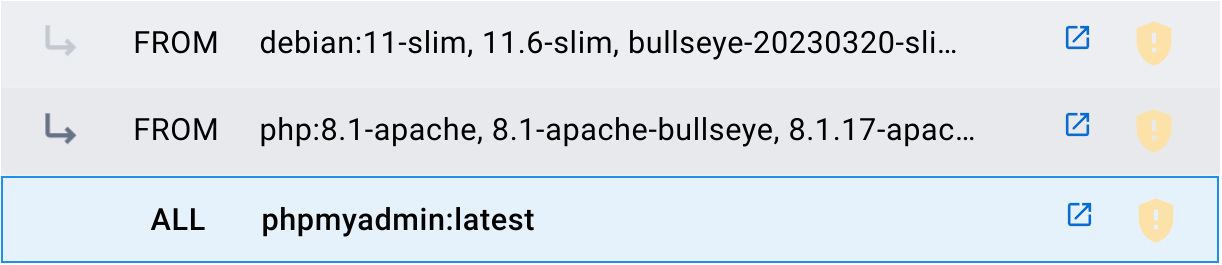
\includegraphics[width=0.9\linewidth]{img/docker/imagen1.png}
    \captionof{figure}{Jerarquía de imágenes usadas por PHPMyAdmin. \href{https://hub.docker.com/layers/library/phpmyadmin/latest/images/sha256-79e38dd8b2ab0e92505aa92040fa49dce4fa921a977b6ce4d030a63b4f120009?context=explore}{Fuente}}
\end{center}

A las imágenes creadas se les suele añadir etiquetas (\textbf{tags}) para diferenciar versiones o características internas. Cada creador determina las etiquetas que le interesa crear. Por ejemplo:
\begin{itemize}
    \item \textbf{latest}: Se le denomina a la última imagen creada.
    \item php:\textbf{8.1-apache}: Indica que en esta imagen PHP la versión es la 8.1 y además cuenta con Apache.
\end{itemize}

Podemos utilizar imágenes públicas descargadas a través de un \textbf{\textit{registry}} público, que no es otra cosa que un repositorio de imágenes subidas por la comunidad. El \textit{registry} principal más utilizado es \href{https://hub.docker.com/}{Docker Hub}.

\infobox{\textbf{Las imágenes Docker  pueden ser públicas o privadas y se almacenan en un repositorio llamado \underline{registry}, siendo el más conocido Docker Hub}}

\textbf{Se pueden crear nuestras propias imágenes privadas}, que pueden ser almacenadas en nuestros equipos o a través de un \textbf{registry privado} que podemos crear (también existen servicios de pago).


\subsection{Contenedores Docker}
Un contenedor Docker es un \textbf{entorno de tiempo de ejecución virtualizado donde los usuarios pueden aislar aplicaciones}. Estos contenedores son unidades compactas y portátiles a las que se les puede aplicar un sistema de limitación de recursos.

\infobox{\textbf{Un contenedor se crea a través de una imagen, es la versión ejecutable de la misma que se crea en un entorno virtualizado}}

Un contenedor se crea a través de una imagen y es la versión ejecutable de la misma. Lo que se hace es crear una capa de escritura sobre la imagen inmutable, donde se podrán escribir datos. Se pueden crear un número ilimitados de contenedores haciendo uso de la misma imagen base.

\vspace{-20pt}
\begin{center}
    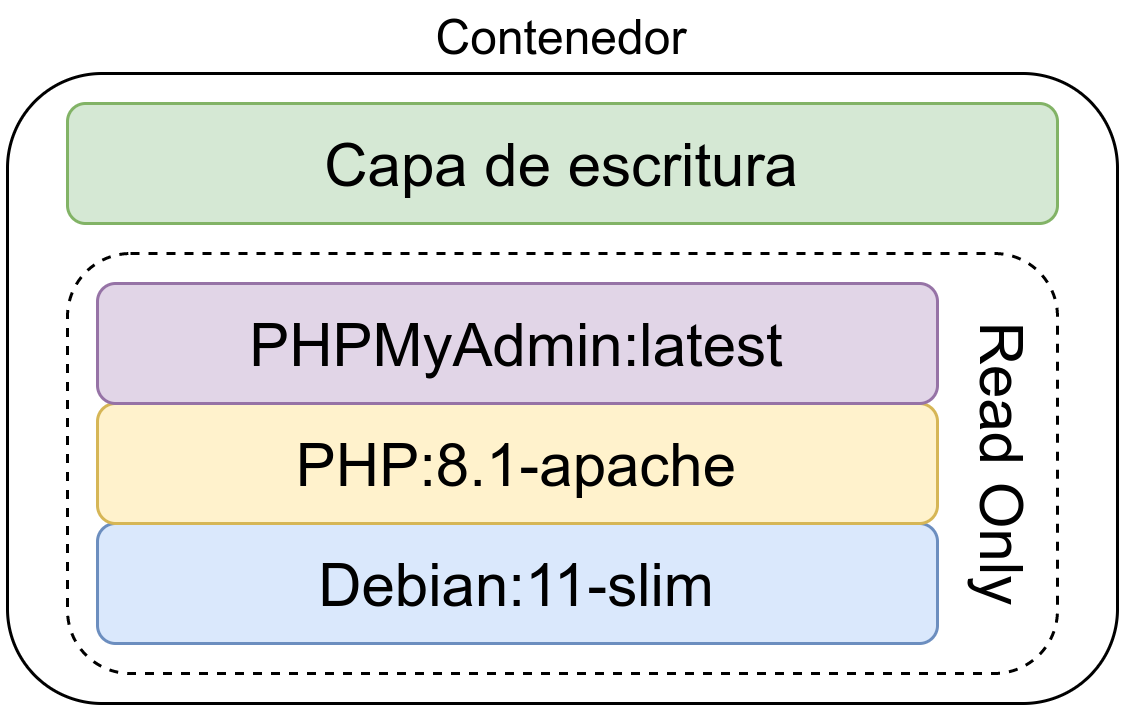
\includegraphics[width=0.6\linewidth]{img/docker/contenedor.png}
    \captionof{figure}{Imagen “interna” de un contenedor}
\end{center}
\vspace{-15pt}

\textbf{La capa de escritura no es persistente} y se pierde al eliminar el contenedor, es decir, \textbf{los datos de un contenedor se eliminan al borrar el contendor}. Para evitar este comportamiento se puede hacer uso de un \hyperlink{volumen_persistente_datos}{volumen persistente de datos}, de esta manera esos datos no se pierden.

\errorbox{\textbf{Los datos creados dentro de un contenedor se borran al eliminar el contenedor}}


\section{Contenedores vs. Máquinas virtuales}

El uso de máquinas virtuales está muy extendido gracias a que cada vez es más sencillo crearlas. Esto no quiere decir que siempre sea la mejor opción, por lo que  se va a realizar una comparativa teniendo en cuenta distintos aspectos a la hora de realizar un desarrollo con máquinas virtuales y con sistemas de contenedores.


\subsection{Infraestructura}

La creación de máquinas virtuales nos permite crear entornos aislados en los que poder instalar el Sistema Operativo que más nos interese y con ello poder instalar el software y los servicios que necesitemos.

Las máquinas virtuales se virtualizan a nivel de hardware, donde debe existir un Sistema Operativo con Hypervisor que permita dicha virtualización. Por otro lado, los contenedores se virtualizan en la capa de aplicación, haciendo que este sistema sea mucho más ligero, permitiendo utilizar esos recursos en los servicios que necesitamos hacer funcionar dentro de los contenedores.

\vspace{-15pt}
\begin{center}
    \includegraphics[width=0.85\linewidth]{img/docker/docker\_vs\_vm.png}
    \captionof{figure}{Infraestructura Máquinas Virtuales vs Docker}
\end{center}
\vspace{-15pt}


En la imagen se puede apreciar una comparativa diferenciando cómo quedaría una infraestructura de 3 aplicaciones levantadas en distintas máquinas virtuales o en distintos contenedores.

Tal como se puede ver en la imagen, \textbf{al tener cada servicio en una máquina virtual separada}, se va a tener que virtualizar todo el Sistema Operativo en el que se encuentre, con el consiguiente \textbf{coste de recursos (memoria RAM y disco duro) y con el coste en tiempo de tener que realizar la configuración y securización del mismo}.

\infobox{\textbf{Usando contenedores la infraestructura se simplifica notáblemente}}

Por otro lado, en un sistema de contenedores, cada contenedor es un servicio aislado, en el que sólo tendremos que preocuparnos (en principio) de configurar sus parámetros.


\subsection{Ventajas durante el desarrollo}

A la hora de desarrollar una aplicación es habitual hacer pruebas utilizando distintas versiones de librerías, \textit{frameworks} o versiones de un mismo lenguaje de programación. De esta manera, podremos ver si nuestra aplicación es compatible.

Cuando se hace uso de una máquina virtual dependemos de las versiones que tiene nuestra distribución y es posible que no podamos instalar nuevas versiones u otras versiones en paralelo.

Por ejemplo, la última versión de PHP actualmente es la 8.2.4 y de Apache la 2.4.56:

\begin{itemize}
    \item En\textbf{ Debian 11} sólo se puede instalar PHP 7.4 y Apache 2.4.54.
    \item En \textbf{Ubuntu 22.04} la versión de PHP es la 8.1 y la de Apache la 2.4.52.
\end{itemize}

Con Docker, podremos levantar contenedores con distintas versiones del servicio que nos interese en paralelo para comprobar si nuestra aplicación/servicio es compatible.

\infobox{\textbf{Con Docker es posible levantar servicios con distintas versiones en paralelo}}

Por otro lado, si un desarrollador quiere utilizar un sistema operativo distinto, no se tendrá que preocupar de si su distribución tiene las mismas versiones. O en el caso de usar Windows/Mac, no tener que estar realizando instalaciones de las versiones concretas.


\subsection{Ventajas durante la puesta en producción}
Ligado al apartado anterior, durante la puesta en producción es obligatorio hacer uso de las mismas versiones utilizadas durante el desarrollo para asegurar la compatibilidad.

\errorbox{\textbf{Para asegurar la compatibilidad en producción, siempre se debe usar la misma versión de los servicios que en desarrollo}}

Si tenemos un servidor que no está actualizado, o en el mismo servidor tenemos distintas aplicaciones que requieren utilizar distintas versiones de software, en un entorno de máquinas virtuales se hace muy complejo, ya que lo habitual será tener que instalar nuevas máquinas virtuales.

\warnbox{\textbf{No siempre es posible tener distintas versiones del mismo software en un mismo servidor}}

En un entorno con contenedores, al igual que se ha comentado antes, esto no es problema.

\subsection{Rapidez en el despliegue}

Ligado a todo lo anterior, realizar el despliegue de un entorno de desarrollo/producción es más rápido utilizando contenedores, sin importar el sistema operativo en el que nos encontremos.

\infobox{\textbf{El despliegue con contenedores es más rápido.}}

Más adelante se verá cómo realizar el despliegue de distintos servicios haciendo uso de un único comando.


\chapter{Docker}

\href{https://www.docker.com/}{Docker} es un proyecto de Software Libre nacido en 2013 que permite realizar el despliegue de aplicaciones y servicios a través de contenedores de manera rápida y sencilla, tal como veremos más adelante.

Estos contenedores proporcionan una capa de abstracción y permiten aislar las aplicaciones del resto del sistema operativo a través del uso de ciertas características del kernel Linux.

Dentro del contenedor, se puede destacar el aislamiento a nivel:

\begin{itemize}
    \item Árbol de procesos
    \item Sistemas de ficheros montados
    \item ID de usuario
    \item Aislamiento de recursos (CPU, memoria, bloques de E/S...)
    \item Red aislada
\end{itemize}

Al igual que sucede con otro tipo de \textit{software},  para que Docker haga uso de todas estas características, está construido haciendo uso de otras aplicaciones y servicios.


\begin{center}
    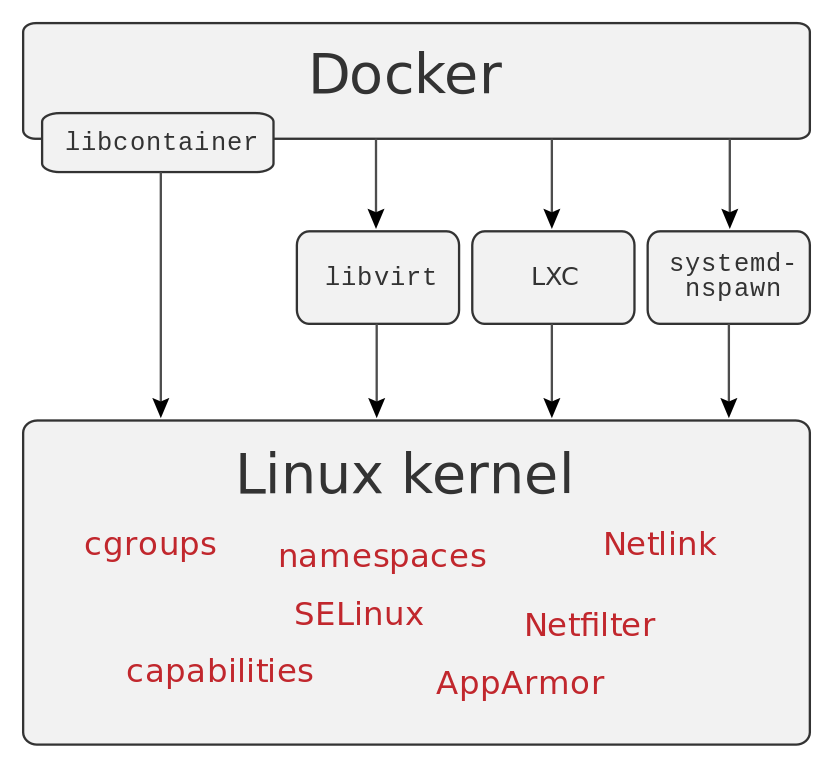
\includegraphics[width=0.75\linewidth]{img/docker/docker_interfaces.png}
    \captionof{figure}{Tecnologías usadas por Docker. Fuente: \href{https://en.wikipedia.org/wiki/File:Docker-linux-interfaces.svg}{Wikipedia}}
\end{center}

En el 2015 la empresa Docker creó la \textbf{\textit{\href{https://en.wikipedia.org/wiki/Open_Container_Initiative}{Open Container Initiative}}}, proyecto actualemente bajo la Linux Foundation, con la intención de diseñar un estándar abierto para la virtualización a nivel de sistema operativo.

\section{Instalación}

Dependiendo del sistema operativo en el que nos encontremos, Docker tiene la opción de instalarse de distintas maneras. En sistemas operativos GNU/Linux cada distribución tiene un paquete para poder realizar la instalación del mismo.

\begin{mycode}{Instalación de Docker en Ubuntu}{console}{}
root@vega:~# apt install docker.io
\end{mycode}

\errorbox{El nombre del paquete en Ubuntu y Debian es \textbf{docker.io}}

En sistemas Windows y MacOS existe la opción de instalar \href{https://docs.docker.com/get-docker/}{Docker Desktop}, una versión que utiliza una máquina virtual para simplificar la instalación en estos sistemas.

\section{Configuración y primeros pasos}

Tras realizar la instalación veremos cómo el servicio Docker ha levantado un interfaz nuevo en nuestra máquina, cuya IP es \textbf{172.17.0.1/16}, siendo el direccionamiento por defecto.

\begin{mycode}{Nueva IP en el equipo}{console}{}
root@vega:~# ip a
...
3: docker0: <BROADCAST,MULTICAST,UP,LOWER_UP> mtu 1500 qdisc noqueue
    link/ether 02:42:9c:1f:e2:90 brd ff:ff:ff:ff:ff:ff
    inet 172.17.0.1/16 brd 172.17.255.255 scope global docker0
      valid_lft forever preferred_lft forever
\end{mycode}

Esta IP hará de \textbf{puente} (similar a lo que sucede con las máquinas virtuales) cuando levantemos contenedores nuevos. Los contenedores estarán dentro de ese direccionamiento 172.17.0.0/16, por lo tanto, aislados de la red principal del equipo.

\infobox{\textbf{Los contenedores que levantemos estarán en la red 172.17.0.0/16}}

El comando \commandbox{docker} tiene muchas opciones, por lo que es recomendable ejecutarlo sin parámetros. De esta manera se pueden ver todas las opciones y una ayuda simplificada para cada una de ellas.

\begin{mycode}{Algunas de las opciones del comando docker}{console}{}
root@vega:~# docker
Usage:  docker [OPTIONS] COMMAND

Management Commands:
builder     Manage builds
completion  Generate the autocompletion script for the specified shell
config      Manage Docker configs
container   Manage containers
context     Manage contexts
image       Manage images
manifest    Manage Docker image manifests and manifest lists
network     Manage networks
node        Manage Swarm nodes
plugin      Manage plugins
secret      Manage Docker secrets
service     Manage services
stack       Manage Docker stacks
swarm       Manage Swarm
system      Manage Docker
trust       Manage trust on Docker images
volume      Manage volumes

Commands:
...
\end{mycode}

Para cada una de estas opciones, se le puede añadir el parámetro \inlineconsole{--help} para mostrar la ayuda. Hay un segundo apartado que se ha cortado, en el que se incluyen más comandos.

Para asegurar que el servicio Docker está funcionando, podemos hacer uso de \commandbox{docker info}, que nos mostrará mucha información acerca del servicio. Pero si lo que queremos es comprobar si tenemos algún contenedor corriendo, es más sencillo hacer \commandbox{docker ps} (que es la versión simplificada de \commandbox{docker container ls} ):

\begin{mycode}{Comprobar estado de Docker y contenedores levantados}{console}{}
root@vega:~# docker ps
CONTAINER ID   IMAGE     COMMAND   CREATED   STATUS    PORTS     NAMES

root@vega:~# docker container ls
CONTAINER ID   IMAGE     COMMAND   CREATED   STATUS    PORTS     NAMES
\end{mycode}

En este caso, como no hay ningún contenedor levantado, sólo muestra las cabeceras de las columnas del listado.

\section{Levantando nuestro primer contenedor}
Es momento de crear nuestro primer contenedor. Para ello, dado que se está usando la consola, hay que hacer uso del comando \commandbox{docker} con una serie de parámetros. En este caso se ha optado por levantar el servicio \textbf{Apache HTTPD}:

\begin{mycode}{Levantando el primer contenedor}{console}{}
root@vega:~# docker run -p 80:80 httpd
AH00558: httpd: Could not reliably determine the server's ...
AH00558: httpd: Could not reliably determine the server's ...
[Fri Mar 24 18:25:14.194246 2023] [mpm_event:notice] ...
[Fri Mar 24 18:25:14.194347 2023] [core:notice] [pid  ...
172.17.0.1 - - [24/Mar/2023:18:25:41 +0000] "GET / HTTP/1.1" 304 -
\end{mycode}

Vemos los logs del servicio Apache al arrancar y si vamos al navegador a la dirección \href{http://localhost}{http://localhost} muestra lo siguiente:

\begin{center}
    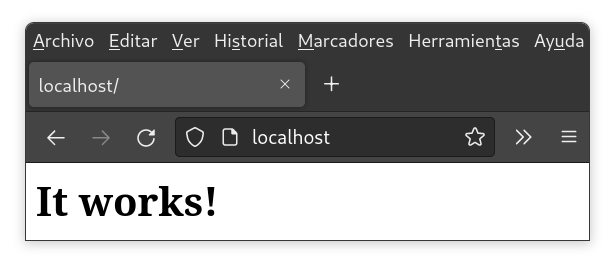
\includegraphics[width=0.6\linewidth]{img/docker/apache.png}
\end{center}

Y para entender lo que hace el comando, los parámetros son:
\begin{itemize}
    \item \textbf{docker}: Cliente de consola para hacer uso de Docker.
    \item \textbf{run}: Ejecuta un comando en un nuevo contenedor (y si no existe lo crea).
    \item \textbf{-p 80:80}: Publica en el puerto 80 del servidor el puerto 80 utilizado en el contenedor. Se puede pensar que es como hacer un \textbf{port-forward} en un firewall.
    \item \textbf{httpd}: Es la \textbf{imagen} del contenedor que se va a arrancar. En este caso, la imagen del servidor \href{https://hub.docker.com/_/httpd}{Apache HTTPD}.
\end{itemize}

Y si vemos qué muestra el estado de docker, vemos cómo aparece el contenedor levantado.

\begin{mycode}{Comprobar estado de Docker y contenedores levantados}{console}{{\scriptsize }}
root@vega:~# docker ps
CONTAINER ID   IMAGE     COMMAND       CREATED         STATUS         PORTS               NAMES
a1c3362b0d6c   httpd     "httpd-..."   3 seconds ago   Up 2 seconds   0.0.0.0:80->80/tcp  great
\end{mycode}

En la columna PORTS se puede apreciar cómo aparece que se ha levantado el puerto  \textbf{ \texttt{0.0.0.0:80} } (escucha en el puerto 80 para cualquier IP del sistema operativo) que es una redirección al puerto \textbf{\texttt{80/TCP}} interno del contenedor.


\section{Contenedores en \textit{background} y más opciones}
Tal como se puede ver en el ejemplo anterior, el contenedor se queda en primer plano, viendo los logs del Apache. Esto para ver qué es lo que está sucendiendo durante el desarrollo puede ser útil, pero lo ideal es que el contenedor arranque en modo \textbf{\textit{background}}, y cuando necesitemos vayamos a ver los logs.


A continuación se va a arrancar un nuevo contenedor de Apache con nuevos parámetros:
\begin{mycode}{Crear un contenedor Web en el puerto 8080}{console}{}
root@vega:~# docker run --name mi-apache -d -p 8080:80 httpd
\end{mycode}

Los nuevos parámetros son:
\begin{itemize}
    \item \textbf{\texttt{--name mi-apache}}: De esta manera se le da un nombre al contenedor, para poder identificarlo de manera rápida entre todos los contenedores creados.
    \item \textbf{\texttt{-d}}: Este parámetro es para hacer el \textbf{\textit{detach}} del comando, y de esta manera mandar a \textbf{\textit{background}} la ejecución del contenedor.
    \item \textbf{\texttt{-p 8080:80}}: Publica en el puerto 8080 del servidor el puerto 80 utilizado en el contenedor. Se puede pensar que es como hacer un \textbf{port-forward} en un firewall.
\end{itemize}


\hypertarget{volumen_persistente_datos}{}
\section{Volumen persistente de datos}
Hasta ahora hemos levantado un contenedor a través de una imagen que levanta el servicio Apache, mostrando su página por defecto. Podríamos escribir en el contenedor la página HTML que nos interesase, pero hay que entender que \textbf{los datos de un contenedor desaparecen cuando el contenedor se elimina}.

Para que los cambios realizados dentro de un contenedor se mantengan, tenemos que hacer uso de los denominados \textbf{volúmenes de datos}. Esto no es más que \textbf{hacer un montaje de una ruta del disco duro del sistema operativo dentro de una ruta del contenedor}.


Estos volúmenes que le asignamos al contenedor pueden ser de dos tipos:
\begin{itemize}
    \item \textbf{Sólo lectura}: Nos puede interesar asignar un volumen de sólo lectura cuando le pasamos ficheros de configuración o la propia web que queremos visualizar.
    \item \textbf{Lectura-Escritura}: En este caso se podrá escribir en el volumen. Por ejemplo, el directorio donde una base de datos guarda la información o una web donde deja imágenes subidas por usuarios.
\end{itemize}

De esta manera, tendremos que asignar el número de volúmenes necesarios a cada contenedor dependiendo de la imagen utilizada, el servicio que se levanta y lo que queremos hacer con los datos que le asignemos o generemos en el contenedor.

En la siguiente imagen se puede ver una infraestructura con dos contenedores y dos volúmenes:
\begin{itemize}
    \item \textbf{Contenedor Web}: Se le asigna un volumen en modo \textbf{sólo lectura} cuya ruta original está en \configdir{/opt/www-data}, que dentro del contenedor está en \configdir{/var/www/html}.
    \item \textbf{Contenedor MySQL}: Dado que los datos de la base de datos deben ser guardados, en este caso se le asigna un volumen que permite escritura. Por lo tanto, lo que se crea dentro del contenedor en \configdir{/var/lib/mysql} realmente se estará guardando en el sistema operativo anfitrión en \configdir{/opt/mysql-data}
\end{itemize}
\begin{center}
    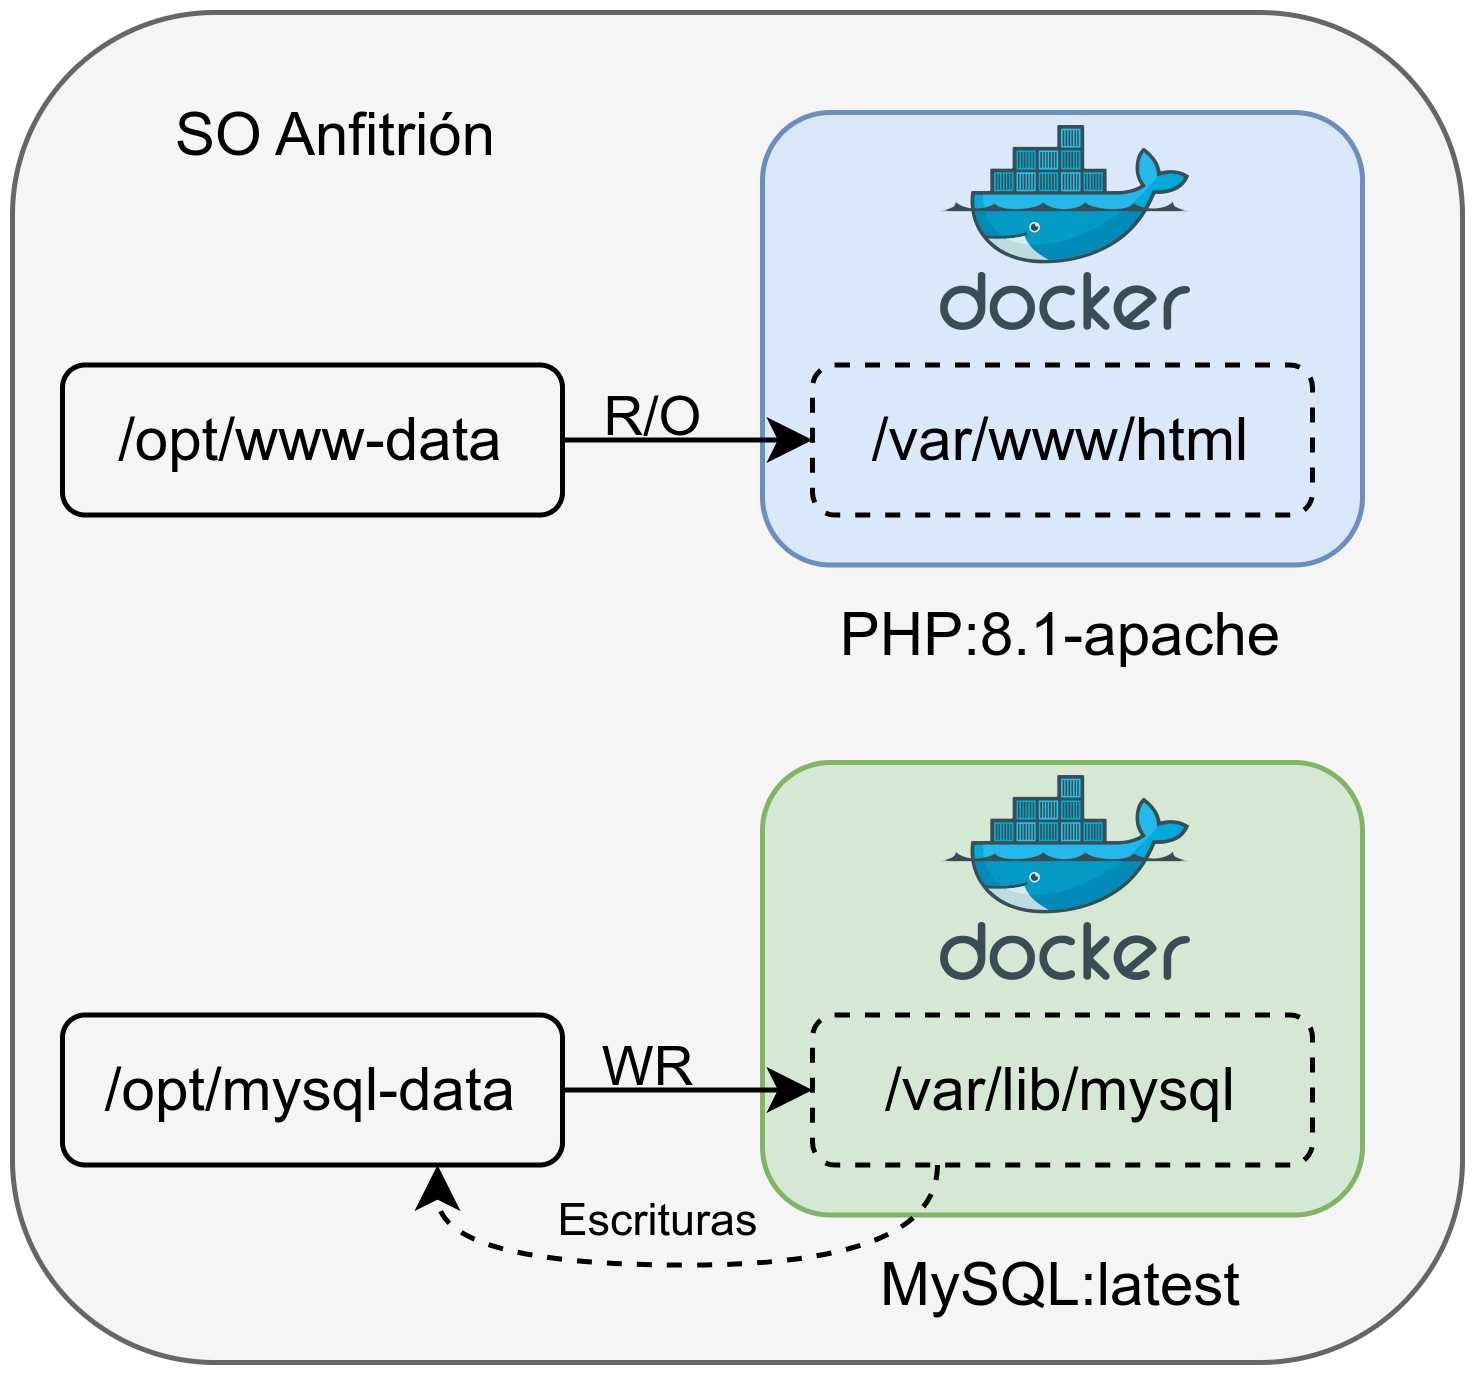
\includegraphics[width=0.65\linewidth]{img/docker/volumes.png}
    \captionof{figure}{Ejemplo de dos volúmenes asignados a distintos contenedores}
\end{center}


\subsection{Añadir volumen de escritura al crear un contenedor}

Al añadir un volumen cuando creamos un contenedor hace que por defecto sea en modo lectura-escritura. Cualquier escritura realizada dentro del contenedor en la ruta especificada va a resultar en que el fichero se creará en la ruta indicada del sistema operativo anfitrión.

\begin{mycode}{Añadir volumen sólo lectura al crear un contenedor}{console}{{\small }}
root@vega:~# ls /opt/mysql-data
root@vega:~# docker run -d -p 3306:3306 --name mi-db \
    -v /opt/mysql-data:/var/lib/mysql \
    -e MYSQL_ROOT_PASSWORD=my-secret-pw \
    mysql:latest
root@vega:~# ls /opt/mysql-data
auto.cnf      client-key.pem      '#innodb_temp'      server-cert.pem   ...
\end{mycode}

Para este ejemplo se ha creado un contenedor usando la imagen de \href{https://hub.docker.com/_/mysql}{MySQL}, al que se le ha asignado un volumen (\textbf{por defecto se asigna permitiendo la escritura}) y un parámetro necesario para realizar la posterior conexión con contraseña.

\begin{itemize}
    \item \textbf{-v /opt/mysql-data:/var/lib/mysql}: A través del parámetro \textbf{-v} se le indica al contenedor que se le va a pasar un volumen. Posteriormente se le indica la ruta del sistema operativo anfitrión \configdir{/opt/mysql-data} que se montará dentro del contenedor en \configdir{/var/lib/mysql}.
    \item \textbf{-e MYSQL\_ROOT\_PASSWORD=my-secret-pw}: El parámetro “\textbf{-e}” sirve para pasarle al contenedor \textbf{variables de entorno}. En este caso, y tal como dice la \href{https://hub.docker.com/_/mysql}{web de la imagen MySQL}, esta es la manera de asignar la contraseña del usuario \textbf{root} durante la inicialización de la base de datos.
\end{itemize}

Tras crear el contenedor, y asegurarnos que está levantado haciendo uso del comando \commandbox{docker ps}, podemos realizar la conexión desde el sistema operativo anfitrión o desde cualquier otro lugar usando la contraseña indicada previamente.

\begin{mycode}{Añadir volumen sólo lectura al crear un contenedor}{console}{{\small }}
root@vega:~# mysql -h127.0.0.1 -uroot -P3306 -p
    Enter password:
    ...
    MySQL [(none)]> show databases;
    +--------------------+
    | Database           |
    +--------------------+
    | information_schema |
    | mysql              |
    | performance_schema |
    | sys                |
    +--------------------+
    4 rows in set (0,007 sec)
\end{mycode}

\subsection{Añadir volumen en modo sólo-lectura}
A continuación se van a explicar los pasos para levantar un contenedor que contiene una web simple creada en PHP, que está alojada en la ruta \configdir{/opt/www-data} del sistema operativo anfitrión.


\begin{mycode}{Añadir volumen sólo lectura al crear un contenedor}{console}{}
root@vega:~# ls /opt/www-data
index.php
root@vega:~# docker run -d -p 80:80 --name mi-web \
    -v /opt/www-data:/var/www/html:ro \
    php:8.2.4-apache
\end{mycode}

El parámetro nuevo asignado en la creación de este contenedor es:
\begin{itemize}
    \item \textbf{-v /opt/www-data:/var/www/html:ro}: Para indicarle que le vamos a asignar un volumen siendo la ruta real en el sistema de ficheros del sistema operativo anfitrión \configdir{/opt/www-data} y la ruta destino \textbf{dentro del contenedor} y que va a ser en modo \textbf{read-only} \configdir{/var/www/html}.
\end{itemize}

Más adelante, cuando veamos \hyperlink{entrar_en_contenedor}{cómo entrar dentro de un contenedor Docker}, se podría usar el comando para ir a la ruta dentro del contenedor y comprobar que efectivamente está en modo sólo-lectura.

\hypertarget{entrar_en_contenedor}{}
\section{Entrar dentro de un contenedor Docker}
Normalmente no suele ser necesario entrar dentro de un contenedor, ya que, tal como se ha dicho antes, cualquier modificación realizada dentro de él se perderá (salvo que sea dentro de un volumen persistente).

Aún así, para realizar pruebas o comprobaciones del correcto funcionamiento de una imagen puede ser interesante entrar dentro de un contenedor. Para ello, el comando a ejecutar es el siguiente:

\begin{mycode}{Acceder a un contenedor}{console}{}
root@vega:~# docker exec -it mi-db /bin/bash
\end{mycode}

Los parámetros utilizados son:
\begin{itemize}
    \item \textbf{exec}: Indicamos que queremos ejecutar un comando dentro de un contenedor que está corriendo.
    \item \textbf{-it}: Son dos parámetros unidos, que sirven para mantener la entrada abierta (modo interactivo) y crear una TTY (consola)
    \item \textbf{mi-db}: Es el nombre del contenedor al que se quiere entrar. También se puede indicar el \textbf{ID} del contenedor.
    \item \textbf{/bin/bash}: el comando que queremos ejecutar. En este caso, una shell \textbf{bash}. En algunos casos esta shell no está instalada y debemos usar \textbf{/bin/sh}
\end{itemize}

Hay que tener en cuenta que dentro de un contenedor está el mínimo software posible para que la aplicación/servicio funcione, por lo que habrá muchos comandos que no existan.


\section{Ciclo de vida de un contenedor Docker}
Un contenedor tiene un ciclo de vida que puede pasar por distintos estados. Para pasar entre estados se debe realizar a través de distintos comandos de Docker.

\begin{center}
    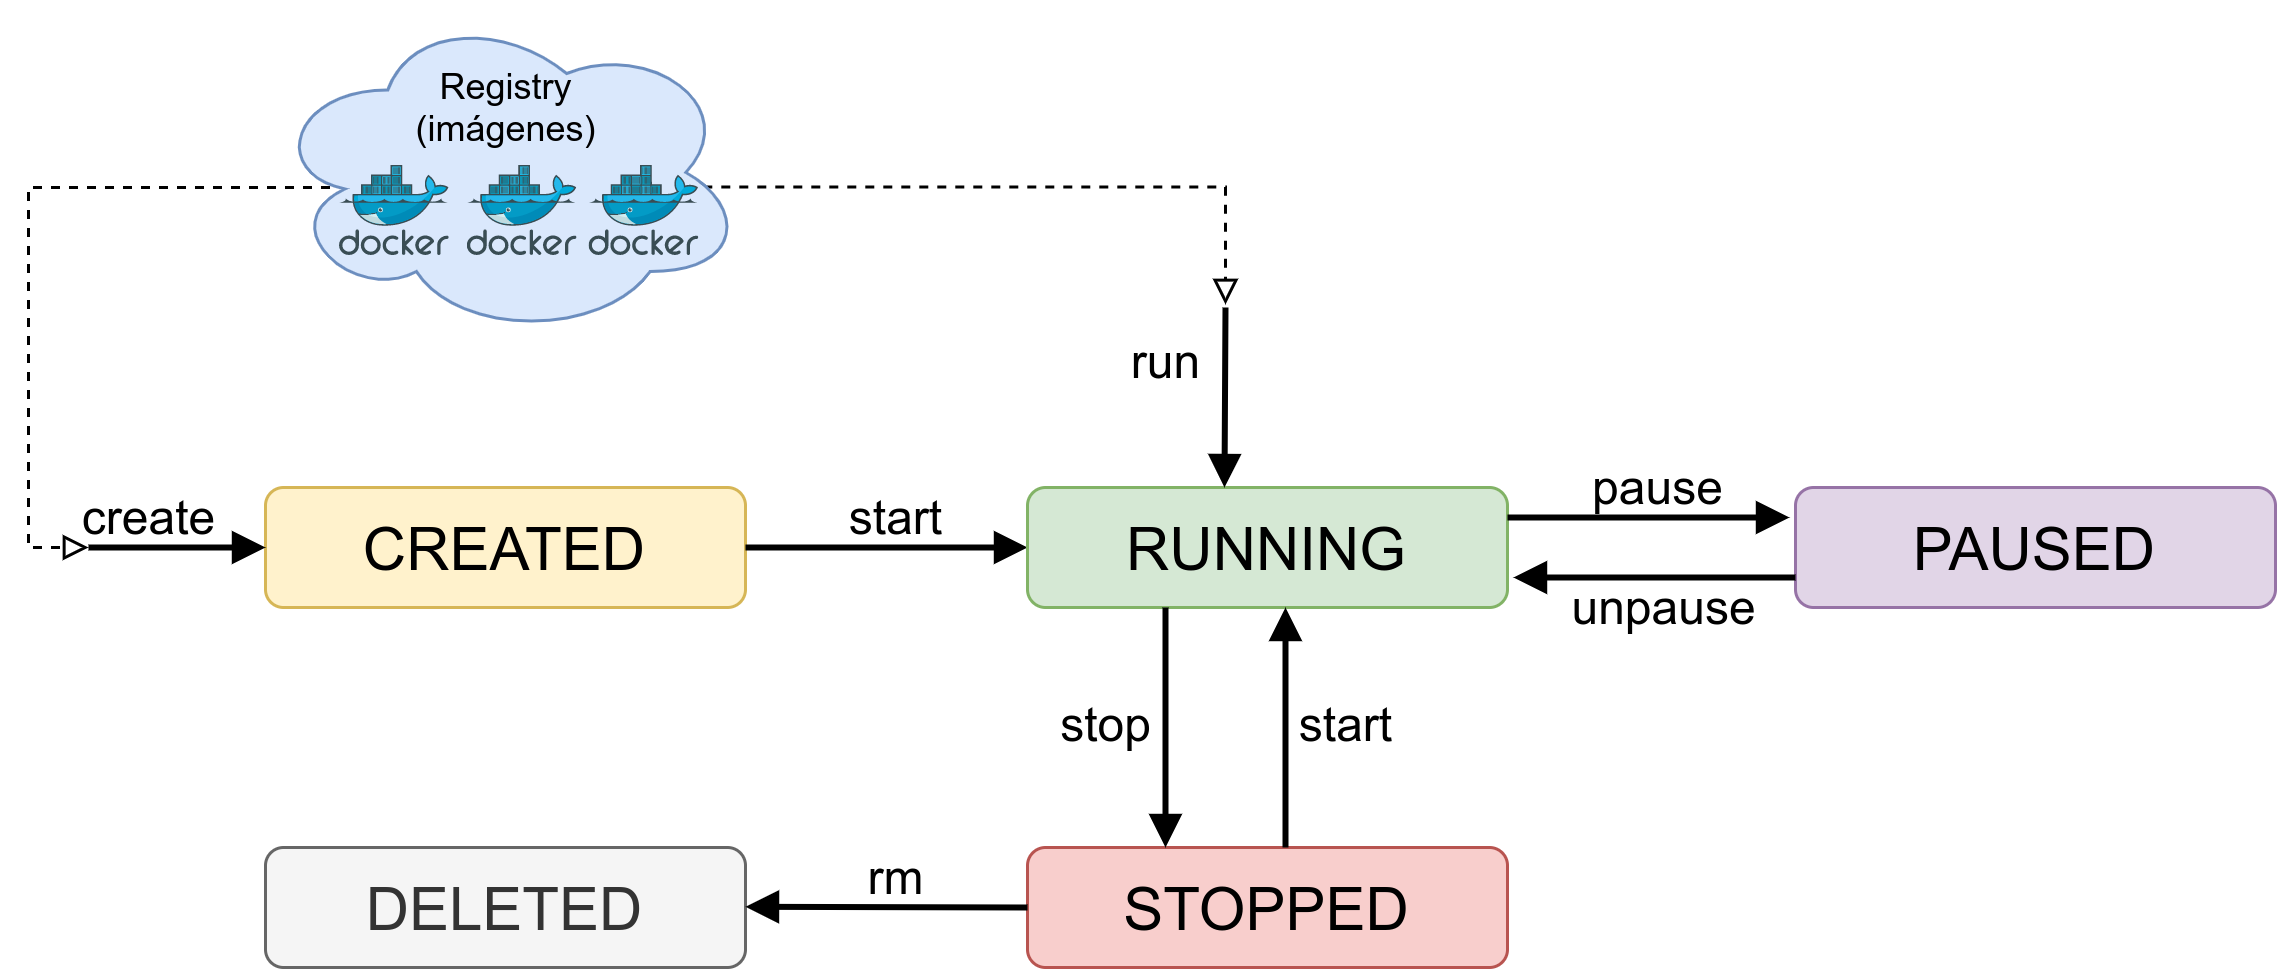
\includegraphics[width=\linewidth]{img/docker/lifecycle.png}
    \captionof{figure}{Estados de un contenedor}
\end{center}

En la imagen se representa los estados más básicos junto con los comandos para pasar entre ellos.


\section{Otros comandos útiles}

Para obtener toda la información de un contenedor, incluido su estado, volúmenes utilizados, puertos, ...

\begin{mycode}{Obtener toda la información de un contenedor}{console}{}
root@vega:~# docker inspect mi-db
\end{mycode}

Listar las imágenes descargadas en local. Al tener las imágenes en local, no hará falta volver a descargarlas, por lo que crear un nuevo contenedor que haga uso de una de ellas será mucho más rápido.

\begin{mycode}{Listado de imágenes en local}{console}{}
root@vega:~# docker image ls
REPOSITORY       TAG            IMAGE ID       CREATED        SIZE
php              8.2.4-apache   de23bf333100   3 days ago     460MB
httpd            latest         192d41583429   3 days ago     145MB
mysql            latest         483a8bc460a9   3 days ago     530MB
\end{mycode}

Borrar una de las imágenes que no se esté utilizando en ningún contenedor.

\begin{mycode}{Borrar una imagen concreta}{console}{}
root@vega:~# docker image rm httpd
\end{mycode}


Cuando un contenedor está en modo \textit{\textbf{detached}} no aparecen los logs, por lo que para poder visualizarlos tenemos un comando especial para ello.
\begin{mycode}{Ver los logs de un contenedor}{console}{}
root@vega:~# docker logs mi-web -f
172.17.0.1 - - [26/Mar/2023:18:05:29 +0000] "GET / HTTP/1.1" 200 248
172.17.0.1 - - [26/Mar/2023:18:05:29 +0000] "GET / HTTP/1.1" 200 248
172.17.0.1 - - [26/Mar/2023:18:05:29 +0000] "GET / HTTP/1.1" 200 248
\end{mycode}


Listar los volúmenes existentes en el sistema. El listado muestra los que se están utilizando en contenedores (activos o parados) o los que se han utilizado en contenedores que ya no existen.

\begin{mycode}{Listar volúmenes}{console}{{\small}}
root@vega:~# docker volume ls
DRIVER    VOLUME NAME
local     0d6c400a6407f5cdea81a2f0158222fdd87d7f3b3e2b5969ca466d743fc71f5c
local     1d2f52018e17af0689e070a55337154c1dd68517c54435ecc24d597f7509d43c
local     6b72797227ef4708ca23ee1dfcb4b651b42eeacefd4166b898407ad4aadda10c
\end{mycode}


Si queremos realizar una limpieza de todos los recursos (contenedores, imágenes,  volúmenes) que no se estén utilizando, se puede utilizar el siguiente comando.
\begin{mycode}{Borrar recursos que no estén activos}{console}{}
root@vega:~# docker system prune -a
WARNING! This will remove:
- all stopped containers
- all networks not used by at least one container
- all images without at least one container associated to them
- all build cache

Are you sure you want to continue? [y/N] y
\end{mycode}

\errorbox{\textbf{El comando anterior hace que se borren contenedores parados}}


Para conocer las estadísticas de uso de cada contenedor.
\begin{mycode}{Ver las estadísticas de los contenedores}{console}{{\scriptsize }}
root@vega:~# docker stats
CONTAINER ID  NAME    CPU %   MEM USAGE / LIMIT     MEM %   NET I/O          BLOCK I/O   PIDS
2fcf97530766  mi-web  0.00%   54.62MiB / 15.47GiB   0.34%   9.44MB / 172kB   0B / 0B     6
413d6e9f590f  mi-db   0.55%   357.9MiB / 15.47GiB   2.26%   319kB / 280B     0B / 0B     38
\end{mycode}


